\section{Conversion Metrics and Development Evidence}
\label{app:e4}
\subsection{Audit aggregation}
For an identity or topology check, the reported F1 is $2TP/(2TP+FP+FN)$. Empty reference/output pairs are excluded when passing; failed or unassessable checks without entity counts receive zero. For a numerical feature or label check with $e>0$ expected values, correct coverage is $\min(1,\max(0,m-i)/e)$, where $m$ is the number of matched values and $i$ the number of matched values outside tolerance. If a failed or unassessable check has no usable expected count, its score is zero; empty passing and inapplicable checks are excluded. Each metric is the arithmetic mean over the included checks from all stages and designs. Repeated stage labels therefore contribute repeated checks; the unique route-endpoint counts in the main text count each design's route labels once. The complete semantic-pass count is computed independently from design-level core verdicts.

\begin{table}[htbp]\centering
\caption{Exact aggregate results for the 600k-budget fixed-cohort retest. Feature/label columns are mean correct coverage under the aggregation above.}
\setlength{\tabcolsep}{3pt}
\begin{tabular}{lrrrrr}\toprule
Method & Core pass & Identity F1 & Topology F1 & Feature & Label\\\midrule
\textbf{R2G} & \textbf{24/24} & \textbf{1.0000} & \textbf{1.0000} & \textbf{100.00\%} & \textbf{100.000\%}\\
GPT-5.6-sol & 0/24 & 1.0000 & 1.0000 & 25.12\% & 13.334\%\\
Claude Opus 5 & 0/24 & 0.7364 & 0.6400 & 8.35\% & 0.087\%\\
Qwen3.7-Max & 0/24 & 0.7239 & 0.6247 & 0.00\% & 0.000\%\\
\bottomrule\end{tabular}

\end{table}

\begin{figure}[htbp]\centering
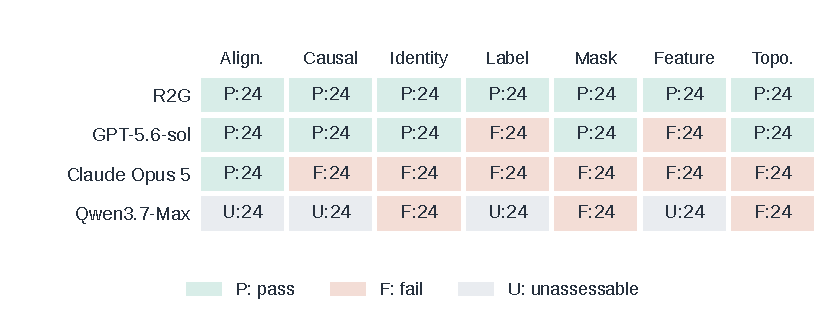
\includegraphics[width=\linewidth]{figures/conversion_core_checks.pdf}
\caption{Design counts in the seven core audit groups. Pass, fail, and unassessable are retained separately. A failure or missing schema may affect several dependent checks; these groups are not independent root causes.}
\end{figure}

The absolute tolerances include 0.0011~$\mu$m for wirelength, $10^{-9}$~pF for ground capacitance, and 0.011~ns for slack, with relative tolerance $10^{-5}$. The audit covers independently available endpoints, not all Liberty attributes, parasitic relations, or physical-label variants.

\subsection{Development budget extension}
The 400k and 600k snapshots below use the same six development designs and the same cumulative development trajectory. They are development metrics, not a comparison of test-set accuracy at two budgets. The 400k snapshots were not retested in this experiment.

\begin{table}[htbp]\centering
\caption{Selected development-program metrics before and after the uniform budget extension. Each arrow denotes 400k $\rightarrow$ 600k ceilings; actual ledger usage can be below the ceiling.}
\setlength{\tabcolsep}{3pt}
\begin{tabular}{lrrrr}\toprule
Model & Identity F1 & Topology F1 & Feature (\%) & Label (\%)\\\midrule
GPT-5.6-sol & 1.000 $\to$ 1.000 & 1.000 $\to$ 1.000 & 18.13 $\to$ 24.80 & 0.000 $\to$ 13.650\\
Claude Opus 5 & 0.684 $\to$ 0.684 & 0.594 $\to$ 0.594 & 8.11 $\to$ 8.11 & 0.118 $\to$ 0.118\\
Qwen3.7-Max & 0.672 $\to$ 0.672 & 0.054 $\to$ 0.577 & 0.00 $\to$ 0.00 & 0.000 $\to$ 0.000\\
\bottomrule\end{tabular}

\end{table}

GPT-5.6-sol improves physical coverage, while Qwen3.7-Max improves topology; Claude Opus 5 retains the same selected program. Additional development can therefore improve individual components without yet completing the graph contract. The main comparison uses one selected program per model, evaluated on all 24 fixed test designs. Test-case diagnosis is performed only after scoring and does not revise these programs or results.

\subsection{Traced conversion case}
Post-test inspection of the selected programs and the \texttt{blinking} design explains the gap between topology and physical supervision (Table~\ref{tab:e4case}). GPT-5.6-sol matches all 211 gates and 644 pins, but none of the 27 expected setup or 27 hold endpoints. Its timing parser primarily expects a slack-before-value pattern, whereas the report contains value-before-slack records such as \texttt{8.54 slack (MET)}; its endpoint resolver also expects an instance/pin form where a report may name only the register instance. These are extraction and joining gaps after successful topology recovery.

\begin{table}[htbp]
\centering
\caption{Representative \texttt{blinking} route-graph audit. Gates/pins show matched identities over expected identities. Label columns show matched values within tolerance over independently expected endpoints. U means unassessable.}
\label{tab:e4case}
\setlength{\tabcolsep}{3pt}
\begin{tabular}{lrrrrrr}\toprule
Method & Gates & Pins & Wirelength & Ground cap. & Setup & Hold\\\midrule
\textbf{R2G} & \textbf{211/211} & \textbf{644/644} & \textbf{209/209} & \textbf{207/207} & \textbf{27/27} & \textbf{27/27}\\
GPT-5.6-sol & 211/211 & 644/644 & 178/209 & 100/207 & 0/27 & 0/27\\
Claude Opus 5 & 184/211 & 563/644 & 2/209 & 0/207 & 0/27 & 0/27\\
Qwen3.7-Max & 184/211 & 466/644 & U & U & U & U\\
\bottomrule\end{tabular}

\end{table}

Claude Opus 5 and Qwen3.7-Max each miss 27 register instances with escaped or special names; their matched pin counts fall to 563 and 466. Missing entities also remove dependent edges. Claude Opus 5's zero initialization produces incorrect physical values and stage-ineligible finite fields; Qwen3.7-Max's missing schemas block physical and label evaluation. R2G preserves all reference identities and matches all independently expected labels in this case: 209 wirelengths, 207 ground capacitances, and 27 values each for setup and hold. Across the 24 designs, the route-graph audit matches 54,322 wirelengths and 54,038 ground capacitances, plus 9,250 values each for setup and hold. The covered wirelength and capacitance endpoints account for 92.3\% and 91.2\% of finite graph values; the remaining values are outside this audit's coverage.
